\documentclass[a4paper,10pt]{article}
\usepackage[utf8]{inputenc}
\usepackage{extsizes}
\usepackage[super,sort&compress,comma]{natbib} 
\usepackage[version=3]{mhchem}
\usepackage[left=1.5cm, right=1.5cm, top=1.785cm, bottom=2.0cm]{geometry}
\usepackage{balance}
\usepackage{mathptmx}
\usepackage{sectsty}
\usepackage{graphicx} 
\usepackage{lastpage}
\usepackage[format=plain,justification=justified,singlelinecheck=false,font={stretch=1.125,small,sf},labelfont=bf,labelsep=space]{caption}
\usepackage{float}
\usepackage{fancyhdr}
\usepackage{fnpos}
\usepackage[english]{babel}
\addto{\captionsenglish}{%
  \renewcommand{\refname}{Notes and references}
}
\usepackage{array}
\usepackage{droidsans}
\usepackage{charter}
\usepackage[T1]{fontenc}
\usepackage[usenames,dvipsnames]{xcolor}
\usepackage{setspace}
\usepackage[compact]{titlesec}
\usepackage{hyperref}
\usepackage{array,longtable}
\usepackage{supertabular,booktabs}
\linespread{2.0}

%opening
\title{Phase stability in nickel phosphides at high pressures}
\author{Talgat M.~Inerbaev$^{*ab}$, Nursultan Sagatov$^{ac}$, Dinara Sagatova$^{ac}$, Pavel N.  Gavryushkin$^{ac}$,  \\ 
Abdirash T. Akilbekov$^{b}$, and Konstantin D. Litasov$^{de}$ \\
\vspace{0pt}\\
\textit{$^{a}$~Sobolev Institute of Geology and Mineralogy, Siberian Branch of the }\\
\textit{ Russian Academy of Sciences, Novosibirsk, 630090 Russia.}\\
\textit{$^{b}$~L. N. Gumilyov Eurasian National University, Nur-Sultan, 010008 Kazakhstan.}\\
\textit{$^{c}$~Novosibirsk State University, Novosibirsk, 630090 Russia.}\\
\textit{$^{d}$~Vereshchagin Institute for High Pressure Physics, Russian Academy of Sciences, }\\
\textit{Moscow, 108840, Russia.}\\
\textit{$^{e}$~Fersman Mineralogical Museum Russian Academy of Sciences, Moscow, Russia.}\\
* Corresponding Author: inerbaevtm@igm.nsc.ru
}

\date{}
\begin{document}

\maketitle

%\begin{abstract}
{\Large{Supporting Information}}
%\end{abstract}
\newpage
\subsection{Phonon spectra for predicted Ni--P structures}

\begin{figure}[h]
 \centering
 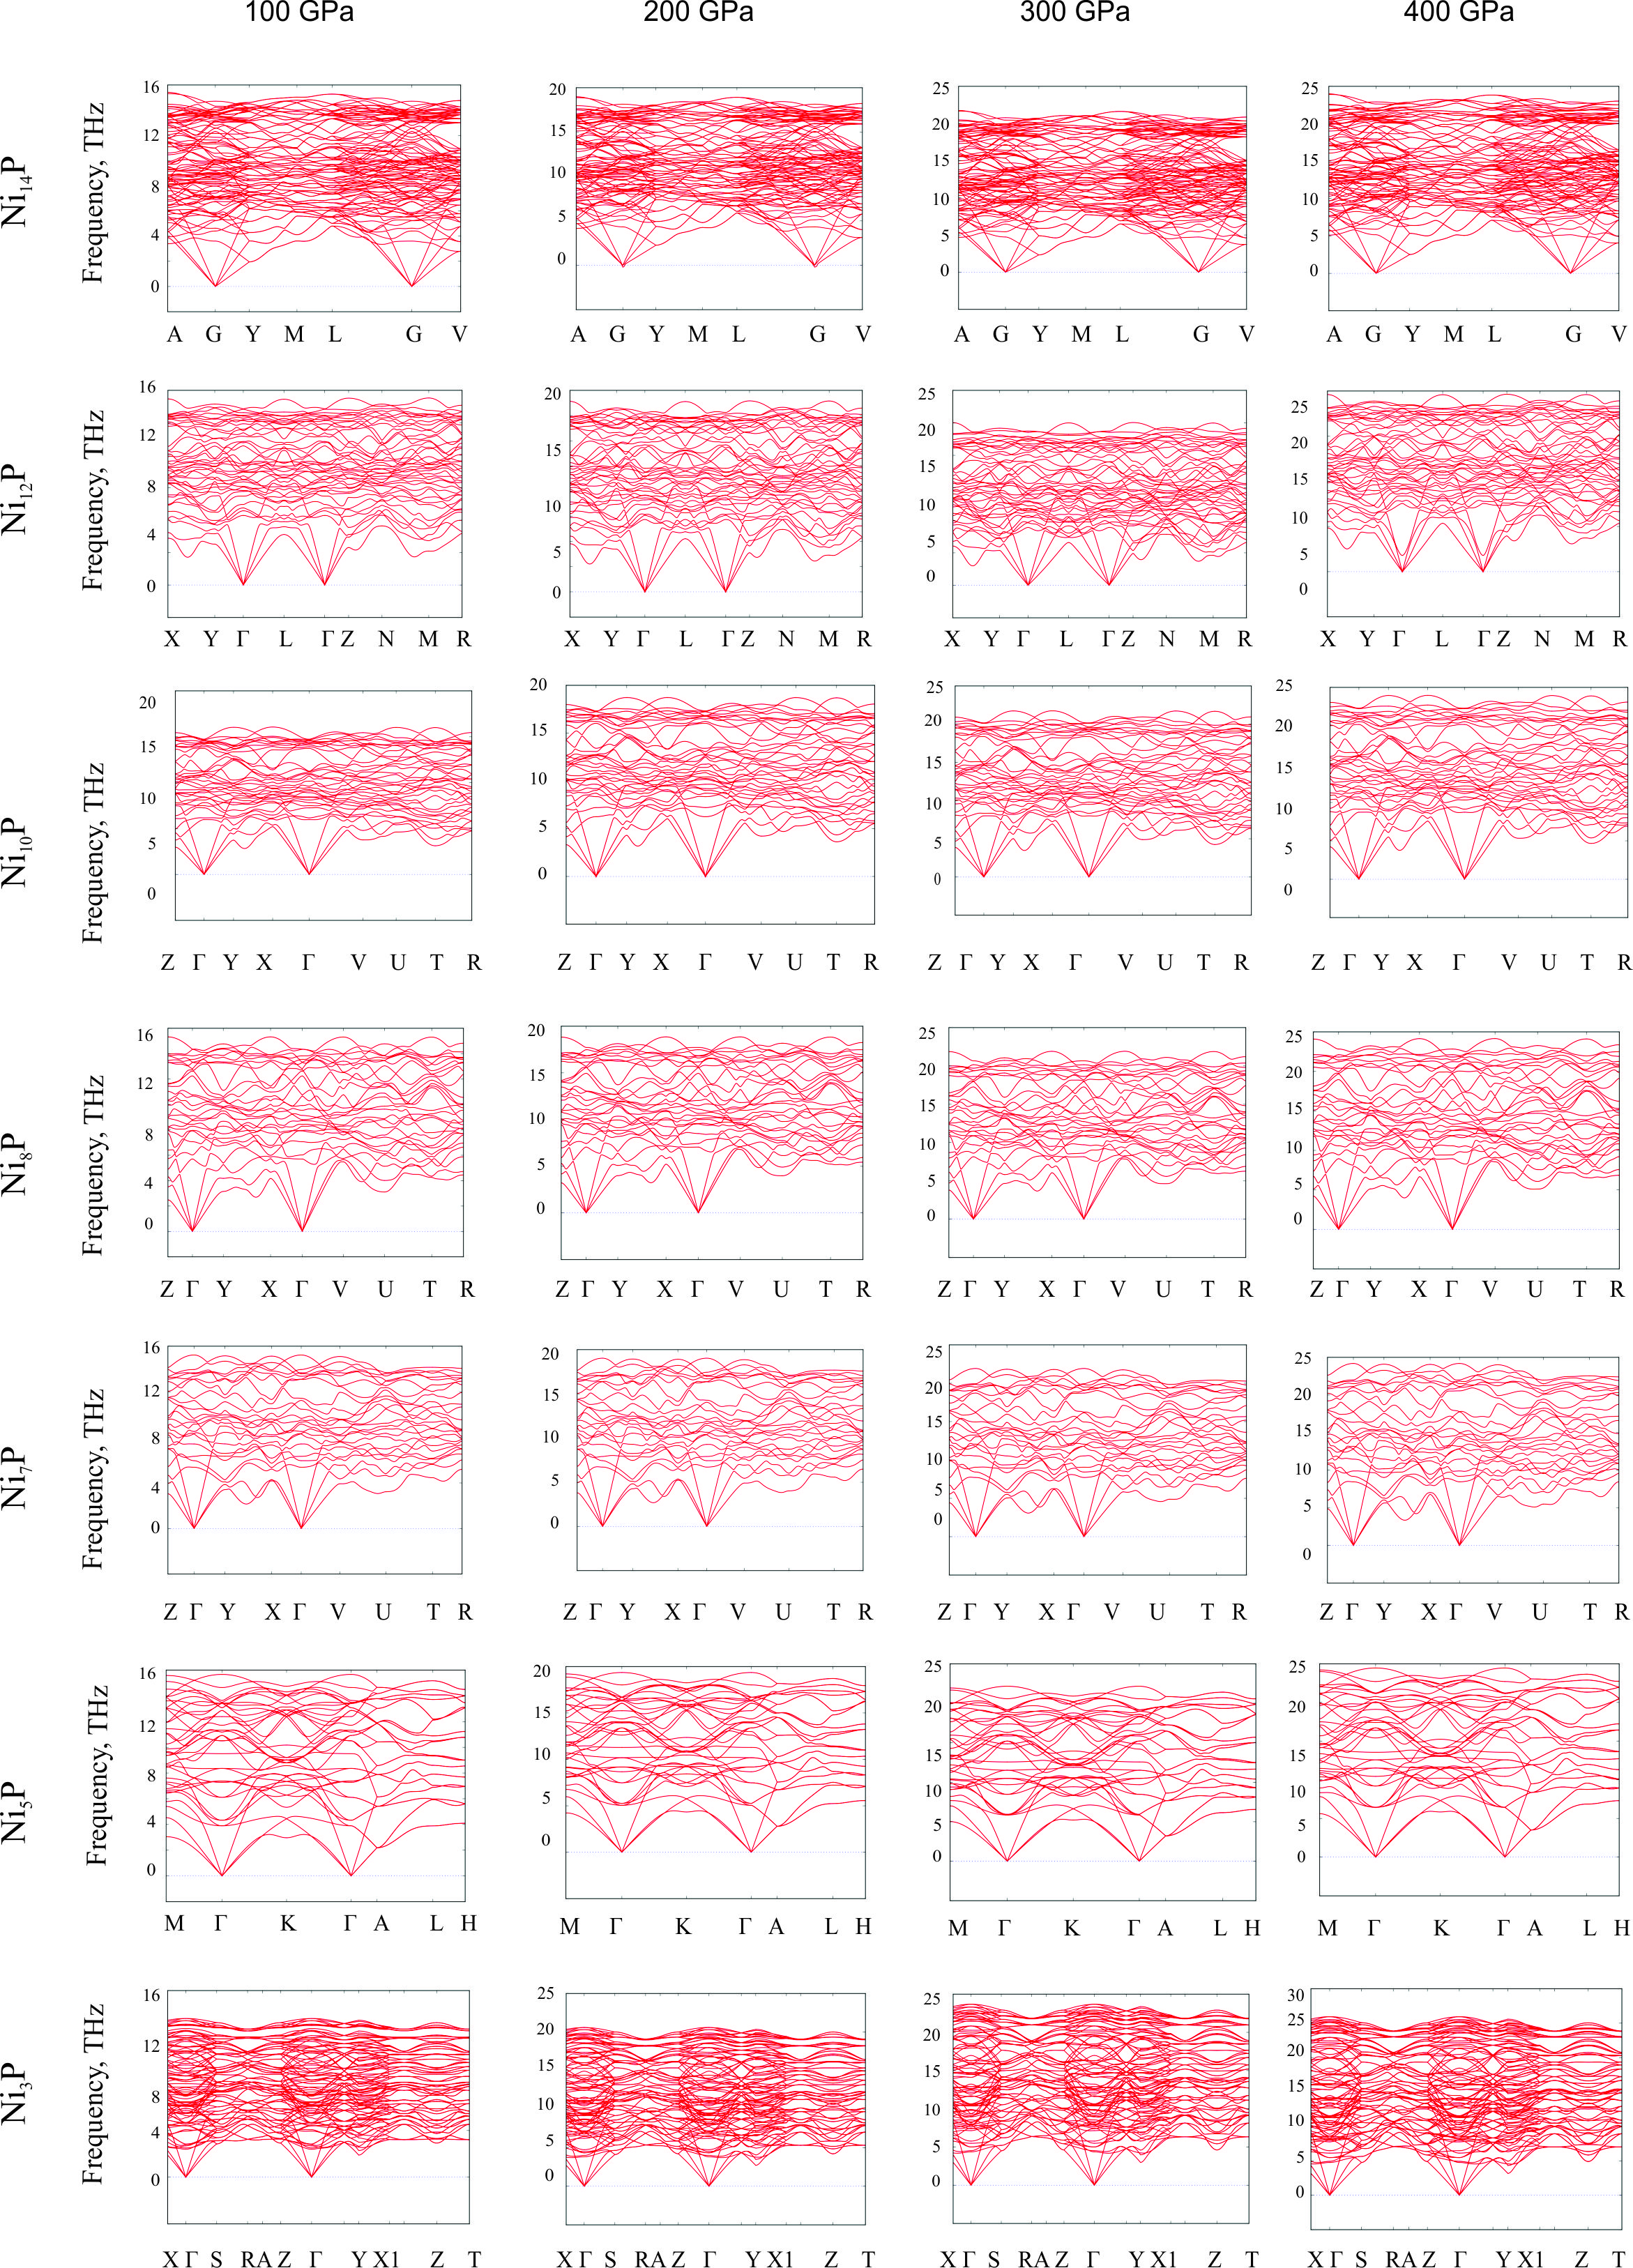
\includegraphics[width=0.75\textwidth]{Phonon-Dispersion.jpg} %[height=6cm]
 \caption{Calculated phonon spectra for predicted Ni--P compounds.}
 \label{phonon-disp}
\end{figure}


\subsection{Elementary substances of Ni and P}
Before exploring the binary Ni-P system, we examined each of the components separately. 
Nickel crystallizes in the face-centered-cubic structure,~\cite{Ni-structure-PhysRev.25.753} and no experimentally structural phase transitions are found in it.
In the case of phosphorus, several pressure-induced structural phase transitions are experimentally observed. 
The most stable form at ambient conditions is the so-called black phosphorus which has the A17 (orthorhombic, space group: {\textit {Cmca}}) structure.~\cite{Black_Phosphorous_1965}
It has been well known that the A17 structure transforms to the A7 ~rhombohedral: {\textit{R$\bar{3}$m}}) structure at 5~GPa and further into the simple cubic (sc: $Pm\bar{3}m$) structure at 10~GPa.~\cite{Jamieson1291,Kikegawa-1983-phosphorous}
A phase transition from the simple cubic to the simple hexagonal structure was observed at 137 GPa via an intermediate phase P-IV.~\cite{Akahama-1999-PhysRevB.59.8520} 
At pressure ~260 GPa hexagonal structure transforms to the body-centered cubic structure~\cite{Akahama-2000-PhysRevB.61.3139} Later it was shown that this structure forms a 2$\times$2$\times$2 superlattice of the bcc structure [c$I$16 (space group: {\textit{I-43d)}}].~\cite{Sugimoto-2012-PhysRevB.86.024109}
Phase P-IV has an incommensurately-modulated   crystal   structure   described   by   the   four-dimensional   superspace   group {\textit{Cmmm}}(00$\gamma$)$s$00.\cite{Fujihisa-2007-PhysRevLett.98.175501,Marques-2008-PhysRevB.78.054120}
In the present study, we approximated the P-IV phase with the eight-atom-cell commensurate structure of $Cmcm$ symmetry.\cite{Marques-2008-PhysRevB.78.054120} 

The calculated dependencies of enthalpy on pressure at 0~K are presented in Fig.~S\ref{phosphorous:enthalpy} 
The theoretical phase diagram qualitatively agrees with the sequence of phase transformations in phosphorus crystals. Some quantitative difference is caused, on the one hand, by the neglect of thermal effects, on the other hand, the difference between the calculated enthalpy values of bcc and I-43$d$ phases in the pressure range of 250-300 GPa is small. 
It does not exceed 0.02 eV per formula unit, which is consistent with the experiment where a sluggish phase transition was observed with the coexistence of these phases in a wide pressure range of 262-322~GPa.~\cite{Sugimoto-2012-PhysRevB.86.024109}
The data obtained were used further to calculate the enthalpy of formation of various crystalline modifications of the Ni--P system.

\begin{figure}[h]
 \centering
 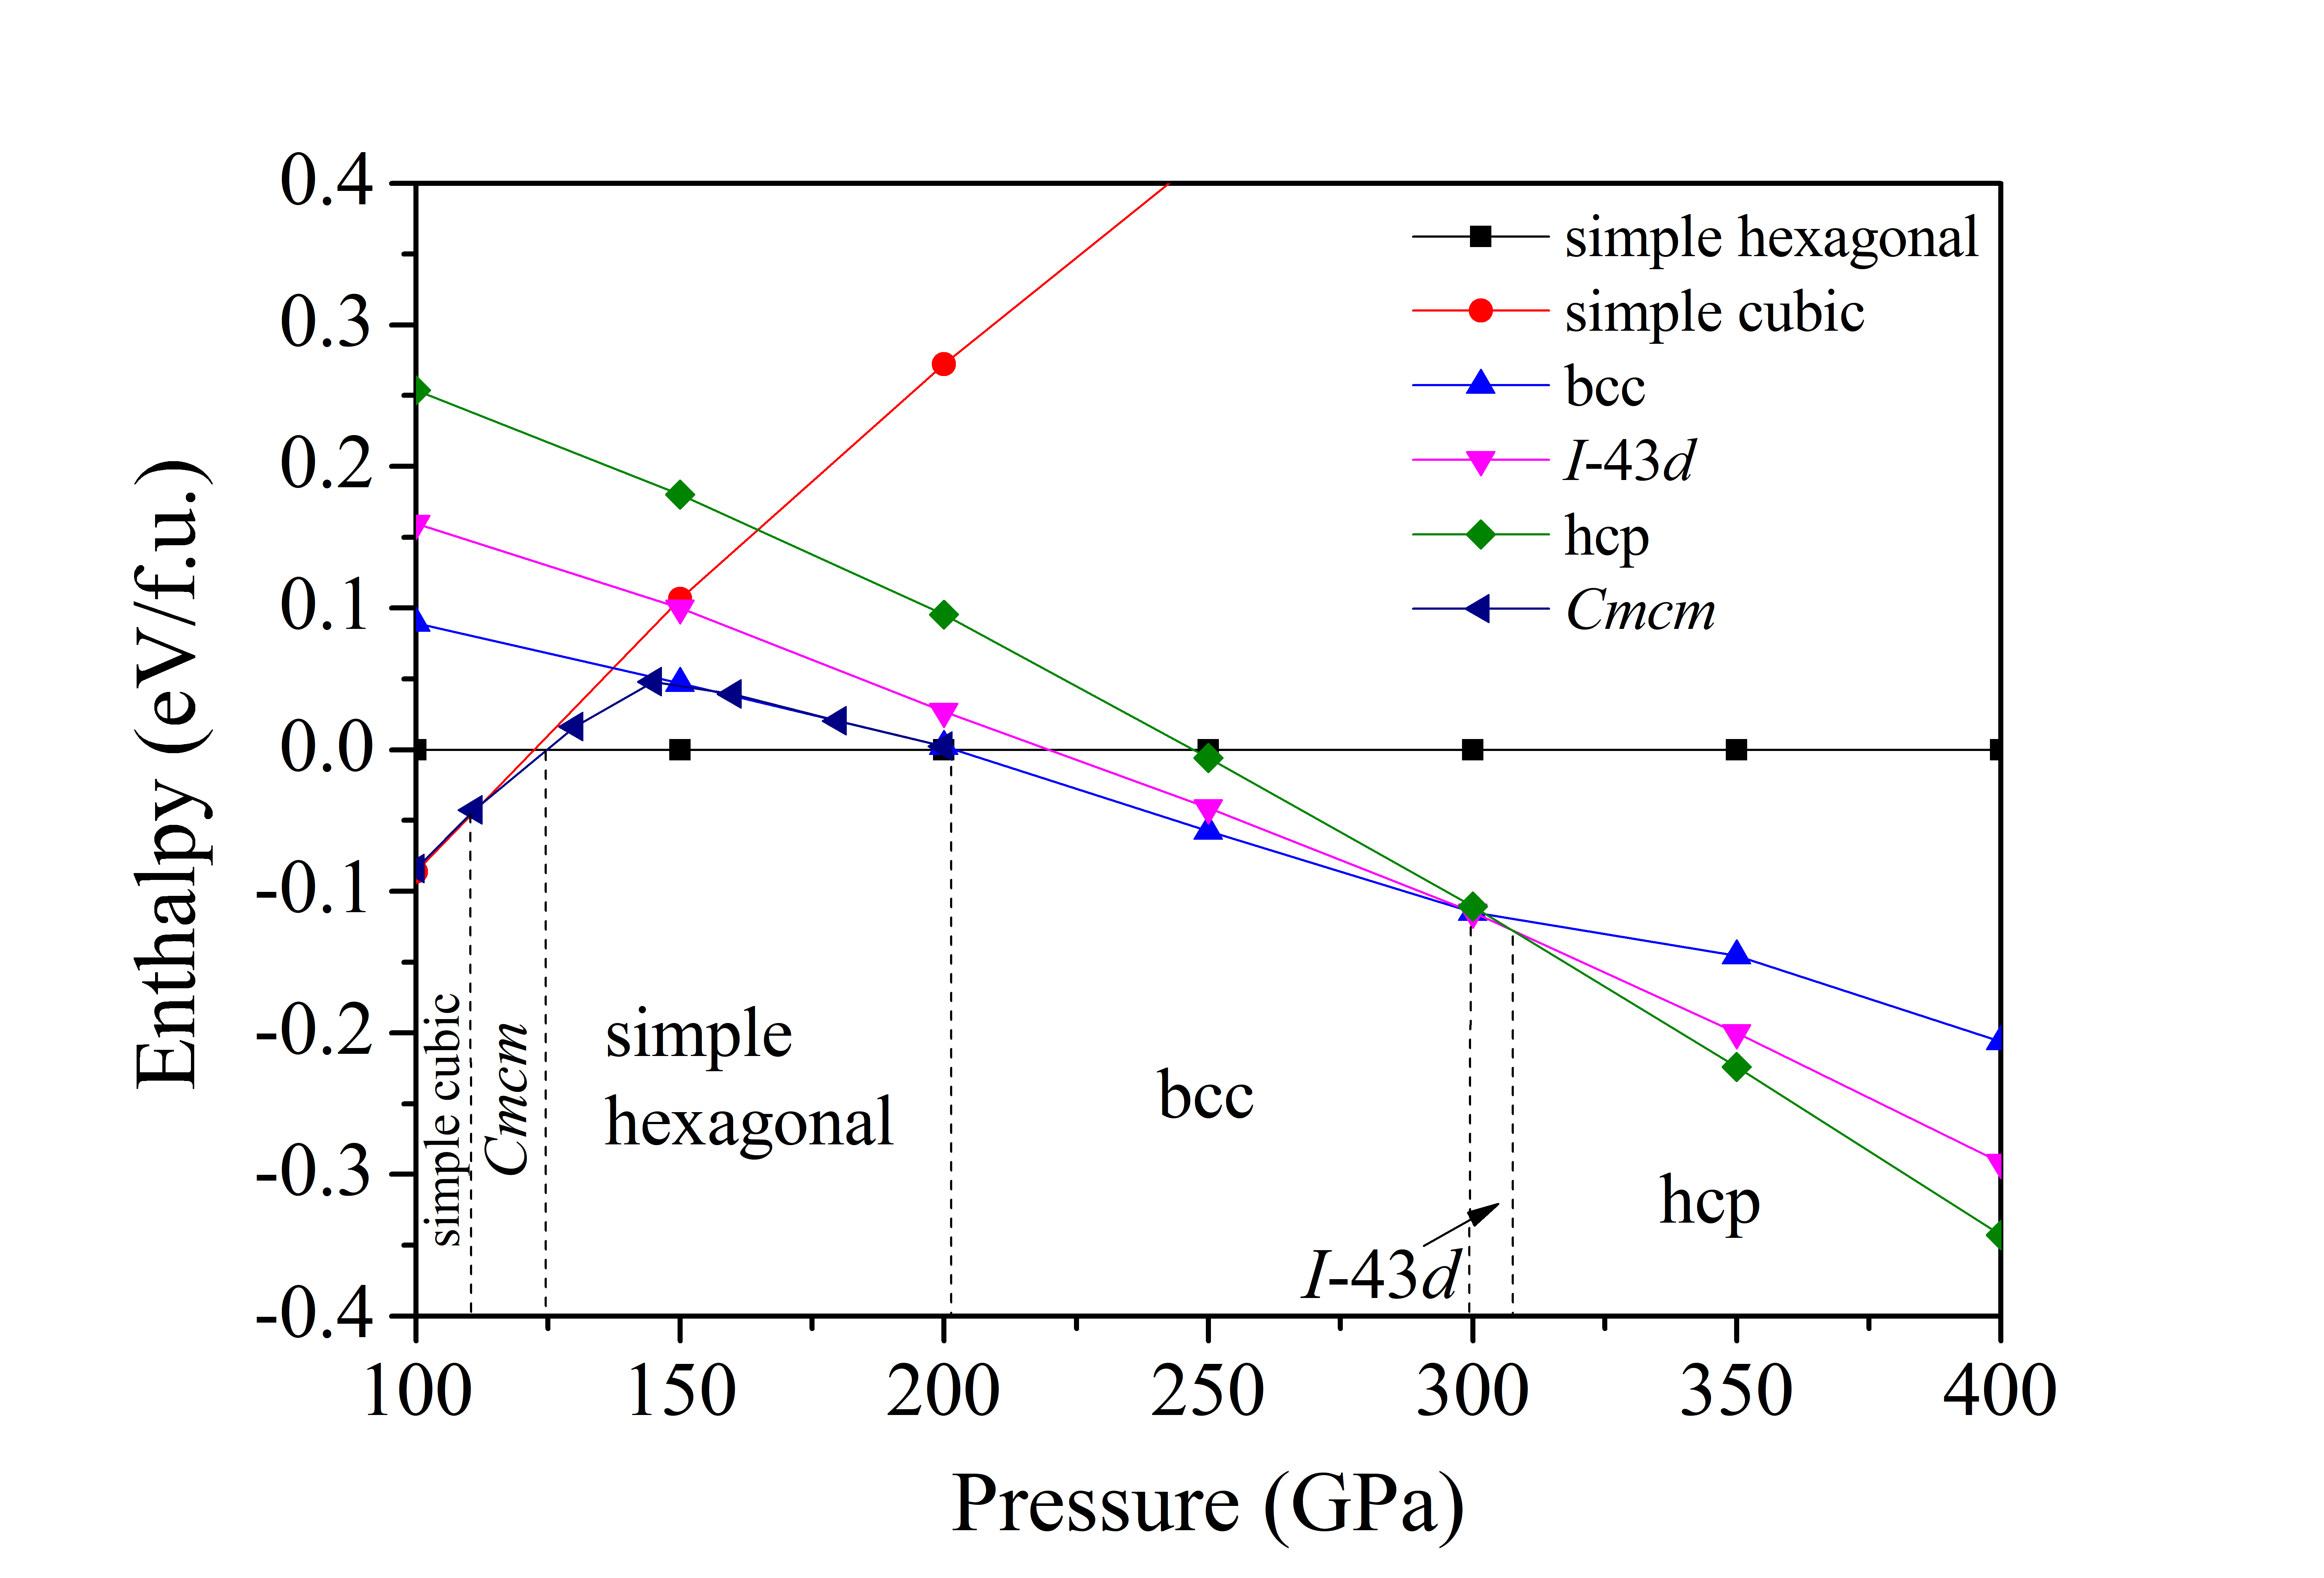
\includegraphics[width=0.9\textwidth]{phosphorus_v1.png} %[height=6cm]
 \caption{Pressure phase diagram of the elementary P.}
 \label{phosphorous:enthalpy}
\end{figure}

\bibliography{NiP} %You need to replace "rsc" on this line with the name of your .bib file
\bibliographystyle{rsc} %the RSC's .bst file


\end{document}
